% !TEX root = ./report.tex

\documentclass[a4paper, 12pt]{extreport}
\usepackage[utf8x]{inputenc}
\usepackage[english,russian]{babel}
\usepackage{shellesc}
\usepackage{amssymb,amsfonts,amsmath,mathtext,cite,enumerate,float}
\usepackage{pgfplots}
\usepackage{graphicx}
\usepackage{svg}
\usepackage[off]{svg-extract}
\svgsetup{clean=true}
\usepackage{tocloft}
\usepackage{listings}
\usepackage{caption}
\usepackage{tempora}
\usepackage{titlesec}
\usepackage{setspace}
\usepackage{geometry}
\usepackage{indentfirst}
\usepackage{pdfpages}
\usepackage{enumerate,letltxmacro}
\usepackage{threeparttable}
\usepackage[hidelinks]{hyperref}
\usepackage{flafter}
\usepackage{enumitem}
\usepackage{multirow}
\usepackage{longtable}
\usepackage[toc]{appendix}
\usepackage{wrapfig}
\usepackage{zref-totpages}

\usepackage[figure,table]{totalcount}
\usepackage{lastpage}

\setlist{nosep}

\newcommand{\ssr}[1]{\begin{center}
		\LARGE\bfseries{#1}
	\end{center} \addcontentsline{toc}{chapter}{#1}  }

\makeatletter
\renewcommand\LARGE{\@setfontsize\LARGE{22pt}{20}}
\renewcommand\Large{\@setfontsize\Large{20pt}{20}}
\renewcommand\large{\@setfontsize\large{16pt}{20}}
\makeatother
\RequirePackage{titlesec}
\titleformat{\chapter}[block]{\hspace{\parindent}\large\bfseries}{\thechapter}{0.5em}{\large\bfseries\raggedright}
\titleformat{name=\chapter,numberless}[block]{\hspace{\parindent}}{}{0pt}{\large\bfseries\centering}
\titleformat{\section}[block]{\hspace{\parindent}\large\bfseries}{\thesection}{0.5em}{\large\bfseries\raggedright}
\titleformat{\subsection}[block]{\hspace{\parindent}\large\bfseries}{\thesubsection}{0.5em}{\large\bfseries\raggedright}
\titleformat{\subsubsection}[block]{\hspace{\parindent}\large\bfseries}{\thesubsection}{0.5em}{\large\bfseries\raggedright}
\titlespacing{\chapter}{12.5mm}{-22pt}{10pt}
\titlespacing{\section}{12.5mm}{10pt}{10pt}
\titlespacing{\subsection}{12.5mm}{10pt}{10pt}
\titlespacing{\subsubsection}{12.5mm}{10pt}{10pt}

\makeatletter
\renewcommand{\@biblabel}[1]{#1.}
\makeatother
%
%\titleformat{\chapter}[hang]{\LARGE\bfseries}{\hspace{1.25cm}\thechapter}{1ex}{\LARGE\bfseries}
%\titleformat{\section}[hang]{\Large\bfseries}{\hspace{1.25cm}\thesection}{1ex}{\Large\bfseries}
%\titleformat{name=\section,numberless}[hang]{\Large\bfseries}{\hspace{1.25cm}}{0pt}{\Large\bfseries}
%\titleformat{\subsection}[hang]{\large\bfseries}{\hspace{1.25cm}\thesubsection}{1ex}{\large\bfseries}
%\titlespacing{\chapter}{0pt}{-\baselineskip}{\baselineskip}
%\titlespacing*{\section}{0pt}{\baselineskip}{\baselineskip}
%\titlespacing*{\subsection}{0pt}{\baselineskip}{\baselineskip}

\geometry{left=30mm}
\geometry{right=10mm}
\geometry{top=20mm}
\geometry{bottom=20mm}

\onehalfspacing

\renewcommand{\theenumi}{\arabic{enumi}}
\renewcommand{\labelenumi}{\arabic{enumi}\text{)}}
\renewcommand{\theenumii}{.\arabic{enumii}}
\renewcommand{\labelenumii}{\asbuk{enumii}\text{)}}
\renewcommand{\theenumiii}{.\arabic{enumiii}}
\renewcommand{\labelenumiii}{\arabic{enumi}.\arabic{enumii}.\arabic{enumiii}.}

\renewcommand{\cftchapleader}{\cftdotfill{\cftdotsep}}

\addto\captionsrussian{\renewcommand{\figurename}{Рисунок}}
\DeclareCaptionLabelSeparator{dash}{~---~}
\captionsetup{labelsep=dash}

\DeclareCaptionFormat{fmt}{\parbox{\linewidth}{#1#2#3}}
\captionsetup{justification=raggedleft,format=fmt,position=bottom}
\captionsetup[figure]{justification=centering,format=default,labelsep=dash}

\graphicspath{{img/}}%путь к рисункам

\newcommand{\floor}[1]{\lfloor #1 \rfloor}

\lstset{ %
	language=python,                 % выбор языка для подсветки
	basicstyle=\small\sffamily, % размер и начертание шрифта для подсветки кода
	numbers=none,               % где поставить нумерацию строк (слева\справа)
	numberstyle=\tiny,           % размер шрифта для номеров строк
	stepnumber=1,                   % размер шага между двумя номерами строк
%	numbersep=5pt,                % как далеко отстоят номера строк от подсвечиваемого кода
	showspaces=false,            % показывать или нет пробелы специальными отступами
	showstringspaces=false,      % показывать или нет пробелы в строках
	showtabs=false,             % показывать или нет табуляцию в строках
	frame=single,              % рисовать рамку вокруг кода
	tabsize=2,                 % размер табуляции по умолчанию равен 2 пробелам
	captionpos=t,              % позиция заголовка вверху [t] или внизу [b] 
	breaklines=true,           % автоматически переносить строки (да\нет)
	breakatwhitespace=false, % переносить строки только если есть пробел
	escapeinside={\#*}{*)},   % если нужно добавить комментарии в коде
	abovecaptionskip=-5pt
}

\pgfplotsset{width=0.85\linewidth, height=0.5\columnwidth}

\linespread{1.3}

\parindent=1.25cm

%\LetLtxMacro\itemold\item
%\renewcommand{\item}{\itemindent0.75cm\itemold}

\def\labelitemi{---}
\setlist[itemize]{leftmargin=1.25cm, itemindent=0.65cm}
\setlist[enumerate]{leftmargin=1.25cm, itemindent=0.55cm}

\newcommand{\specialcell}[2][c]{%
	\begin{tabular}[#1]{@{}c@{}}#2\end{tabular}}

\frenchspacing

\begin{document}


\includepdf[pages={1}]{parts/01_title.pdf}
\setcounter{page}{2}

\ssr{РЕФЕРАТ}

\pagebreak

\begingroup
\renewcommand{\vspace}[2]{}% Gobble 2 arguments after \vspace
\def\contentsname{\begin{center}СОДЕРЖАНИЕ\end{center}}
\tableofcontents
\endgroup

\ssr{ОПРЕДЕЛЕНИЯ}

\pagebreak

\ssr{ОБОЗНАЧЕНИЯ И СОКРАЩЕНИЯ}

В этой расчётно-пояснительной записке применяются следующие сокращения и обозначения.

ПО -- Программное обеспечение.

Алгоритм QWFC (WFC) -- Алгоритм квантового коллапса волновой функции.

\pagebreak

\ssr{ВВЕДЕНИЕ}

\textbf{Компьютерная графика} -- это область информатики, занимающаяся созданием, обработкой и отображением изображений с использованием вычислительных технологий. Она включает в себя как двумерную, так и трёхмерную графику, а также анимацию и визуализацию данных. Актуальность компьютерной графики возрастает с развитием технологий, таких как виртуальная и дополненная реальность, которые требуют высококачественной визуализации для создания реалистичных и интерактивных пользовательских опытов. В современных приложениях, от видеоигр до медицинской визуализации, компьютерная графика играет ключевую роль в представлении информации и взаимодействии с пользователями, что делает её важной областью для исследования и развития.

Целью данного курсового проекта является разработка ПО с пользовательским интерфейсом для генерации и визуализации загородного посёлка. Сцена содержит модели домов, источник света и камеру. Интерфейс пользователя должен позволять задавать параметры для генерации посёлка: размер домов, количество домов, ширина дорог, шаблоны расположения (кварталами или случайно). 

Интерфейс приложения также должен предоставлять возможность для передвижения камеры и источника света.

Для достижения поставленной цели нужно решить следующие задачи:
\begin{itemize}
  \item сравнение существующих алгоритмов процедурной генерации сцены;
  \item сравнение существующих алгоритмов компьютерной графики, использующихся для визуализации трёхмерной модели (сцены);
  \item выбор подходящих алгоритмов для решения поставленных задач;
  \item проектирование архитектуры и графического интерфейса ПО;
  \item выбор средств реализации ПО;
  \item разработка спроектированного ПО;
  \item замер временных характеристик разработанного ПО.
\end{itemize}
\clearpage

\chapter{Аналитическая часть}


\section{Формализация синтезируемой сцены}

Сцена состоит из следующего набора объектов:
\begin{enumerate}
    \item камера;
    \item источник света;
    \item модель загородного посёлка, состоящая из: 
    \begin{itemize}
        \item домов;
        \item дорог;
        \item деревьев.
    \end{itemize}
\end{enumerate}

\subsection*{Камера}

Камера не является видимым объектом сцены. Она характеризуется только своим положением в пространстве и направлением просмотра. Изображение с камеры отображается в пользовательском интерфейсе ПО;

\subsection*{Источник света}

Источник света отображает солнце, поэтому является всенаправленным и всегда находится на сравнительно большом расстоянии от других объектов сцены.

В пользовательском интерфейсе должна быть возможность задать положение источника света путём задания двух углов, которые задают направление, в котором будет находиться источник света относительно центра сцены. 

Также в пользовательском интерфейсе должна быть возможность изменить расстояние, на котором находится источник света относительно центра сцены.

\subsection*{Модель загородного посёлка}

Модель загородного посёлка является основной частью сцены. Сама модель должна генерироваться в соответствии с параметрами, заданными пользователем в пользовательском интерфейсе.

Далее формализуются объекты, входящие в сцену:

\subsubsection*{Ландшафт}

В сцене не подразумевается использование сложного ландшафта, поэтому в качестве ландшафта используется плоское поле зелёного цвета (поле)

\subsubsection*{Дома}

Дома, входящие в сцену состоят из геометрических примитивов, таких как:
\begin{itemize}
    \item кубы;
    \item призмы.
\end{itemize}

Дома имеют простой прямоугольный фундамент разных размеров. В качестве крыши всегда используются призмы.

\subsubsection*{Дороги}

Дороги должны проходить между домами и соединять их в улицы. 

С точки зрения модели, дорогами являются прямоугольники, лежащие на плоскости ландшафта.

\subsubsection*{Деревья}

Деревья также состоят из геометрических примитивов:
\begin{itemize}
    \item параллелепипедов.
\end{itemize}

Все деревья будут представляться дубами, имеющими параллелепипед коричневого цвета в качестве ствола и тёмно-зелёную листву, отображаемую в виде куба.

\subsection*{Расположение объектов на модели}

Основная плоскость является двумерной сеткой.

Пусть ячейка --- это такой блок двумерной сетки который может:
\begin{itemize}
    \item пустовать --- в пределах ячейки нет объектов модели помимо основной плоскости;
    \item быть занят --- в пределах ячейки содержится один или несколько объектов сцены.
\end{itemize}

В одной ячейке не может быть одновременно больше одного типа объектов (дом, дорога, дерево).

Объекты не обязательно должны занимать всю площадь ячейки.

Все дома должны стоять около хотя бы одной дороги.

Считается, что пространство за границей сцены может содержать ячейки любого типа, то есть находится в состоянии неопределённости.


\section{Способы процедурной генерации сцены}

\subsection*{Алгоритм квантового коллапса волновой функции}

Алгоритм квантового коллапса волновой функции (далее - QWFC или WFC) — это метод генерации контента, который используется для создания двумерных и трёхмерных структур, таких как уровни в видеоиграх, текстуры и другие элементы. Он был разработан Максимом Гуминым и основан на концепциях из квантовой механики, хотя и не имеет прямого отношения к физике. \cite{QWFC}

Алгоритм работает путём заполнения сетки, каждая ячейка которой может принять одно из определённых состояний. Для заполнения сетки требуется предопределённый набор правил и приоритетов, который описывает то, какие ячейки могут быть "соседями" других ячеек. Изначально все ячейки находятся в состоянии суперпозиции -- каждая может принять любое состояние (отсюда происходит слово "квантовый" в названии алгоритма). Затем, у случайной ячейки фиксируется одно из состояний (которое также выбирается случайно, но есть возможность задать приоритеты для тех или иных состояний). На основе этой зафиксированной ячейки, обновляется состояние остальной сетки, чтобы учесть появившиеся ограничения. Цикл повторяется, пока сетка не будет заполнена.

Этот алгоритм подходит для выполнения поставленной задачи (генерации загородного посёлка), так как он позволяет нам заполнить заданную плоскость в соответствии с ограничениями, а также предоставляет возможность влиять на результат посредством коэффициентов, которые можно задавать в пользовательском интерфейсе.


\section{Способы описания трёхмерных геометрических моделей на сцене}

Существует три основных типа трёхмерных моделей \cite{CGPaP}:
\begin{enumerate}
    \item \emph{каркасная модель} -- описывает вершины и рёбра между ними;
    \item \emph{поверхностная модель} -- описывает вершины, рёбра и поверхности;
    \item \emph{твердотельная модель} -- описывает ещё и с какой стороны расположен материал;
\end{enumerate}

Для решения поставленной задачи лучше всего подходит поверхностная модель. 
Каркасная модель не позволяет задать свойства плоскостей (такие, как цвет, параметры отражения и блеска), требуемые для правильного восприятия сцены.
Твердотельная модель содержит данные, нужды в которых для достижения цели --- нет.


\section{Сравнение алгоритмов удаления невидимых поверхностей}

Алгоритмы удаления невидимых линий и поверхностей используются в машинной графике для удаления тех объектов (или частей объектов), которые перекрываются другими. Задача удаления невидимых линий и поверхностей является одной из наиболее сложных в машинной графике~\cite{Rogers}.

В этом разделе будут рассмотрены несколько алгоритмов удаления невидимых поверхностей, а для сравнения будут использованы следующие критерии:
\begin{itemize}
    \item необходимость в сортировке объектов сцены;
    \item возможность реализации оптических эффектов;
    \item временная сложность алгоритма в зависимости от: \begin{itemize}
        \item разрешения экрана;
        \item количества граней на сцене.
    \end{itemize}
\end{itemize}

\subsection*{Алгоритм Варнока}

Алгоритм Варнока (или алгоритм художника) основывается на разбиении пространства на области, которые могут быть классифицированы, как сложные и простые.

Под сложной областью подразумевается такая область (часть пространства на экране), которая превышает по размеру один пиксель и в которой возникает любой из следующих случаев:
\begin{itemize}
    \item в область попали несколько объектов;
    \item в область попал один объект, который занимает не всю область.
\end{itemize}

Простой областью, в свою очередь, называются такие области, которые либо не превышают по размеру один пиксель, либо не являются сложными.

Алгоритм рекурсивно делит экранное пространство на области, пока не достигает простых областей, которые могут быть закрашены тем или иным цветом.

Необходимости в сортировке объектов сцены для этого алгоритма нет, однако такая сортировка значительно увеличивает эффективность алгоритма~\cite{Rogers}.

Данный алгоритм не даёт возможности для реализации оптических эффектов.

Сложность алгоритма равна $O(WHN)$, где W --- ширина экрана, H --- высота экрана, N --- количество обрабатываемых граней~\cite{Rogers}.

\subsection*{Трассировка лучей}

Трассировка лучей --- это более сложный и точный метод, который использует физический принцип распространения света. 

В этом методе лучи "выстреливаются" из камеры в сцену, и для каждого луча вычисляется, какие объекты он пересекает. При пересечении луча с объектом, луч может не только остановиться, но и отразиться или преломиться. 

Необходимости в сортировке объектов сцены для этого алгоритма нет.

Трассировка лучей позволяет добиться высокой степени реализма, путём точной симуляции оптических эффектов, однако она требует значительных вычислительных ресурсов.

Сложность алгоритма равна $O(WHN)$, где W --- ширина экрана, H --- высота экрана, N --- количество обрабатываемых граней~\cite{Rogers}. Однако вычислительная сложность данного алгоритма будет значительно выше других из-за дополнительной сложности в обработке каждого трассируемого луча. Эта сложность не отображается в нотации O-большое, так как является константой.

\subsection*{Алгоритм с Z-буфером}

Алгоритм с Z-буфером (или глубинным буфером) --- это один из простейших~\cite{Rogers} методов удаления невидимых поверхностей. 

Он использует дополнительную матрицу глубин, называемую буфером для хранения информации о глубине каждого пикселя на экране. При отрисовке каждого объекта сцены, глубина пикселей этого объекта сравнивается с уже сохраненной в буфере глубиной. Если новый объект ближе к камере, то есть глубина пикселя меньше того, что записано в буфере, его цвет записывается в матрицу цветов пикселей кадра, а его глубина --- в матрицу глубин. 

Этот метод позволяет эффективно обрабатывать сложные сцены и обеспечивает высокую производительность, что позволяет использовать его и при отрисовке сцен в реальном времени.

Необходимости в сортировке объектов сцены для этого метода нет.

Данный алгоритм не даёт возможности для реализации оптических эффектов.

Сложность алгоритма равна $O(WHN)$, где W --- ширина экрана, H --- высота экрана, N --- количество обрабатываемых граней~\cite{Rogers}.

\subsection*{Вывод}

Результаты сравнения алгоритмов удаления невидимых поверхностей представлены в таблице~\ref{tbl:comparison}.

\begin{table}[h!]
    \caption{Таблица результатов сравнения алгоритмов удаления невидимых поверхностей}
    \label{tbl:comparison}
    \begin{tabular}{|l|l|l|l|}
    \hline
    Критерий                                                                             & \begin{tabular}[c]{@{}l@{}}Алгоритм\\ Варнока\end{tabular}                                                  & \begin{tabular}[c]{@{}l@{}}Алгоритм\\ Трассировки\\ Лучей\end{tabular} & \begin{tabular}[c]{@{}l@{}}Алгоритм\\ с Z-буфером\end{tabular} \\ \hline
    \begin{tabular}[c]{@{}l@{}}Необходимость\\ в сортировке граней\end{tabular}          & \begin{tabular}[c]{@{}l@{}}Нет, но сортировка \\ значительно увеличивает \\ производительность\end{tabular} & Нет                                                                    & Нет                                                            \\ \hline
    Временная сложность                                                                  & $O(WHN)$                                                                                                    & $O(WHN)$                                                               & $O(WHN)$                                                       \\ \hline
    \begin{tabular}[c]{@{}l@{}}Возможность реализации\\ оптических эффектов\end{tabular} & Нет                                                                                                         & Да                                                                     & Нет                                                            \\ \hline
    \end{tabular}
    \end{table}

Было принято решение использовать алгоритм с Z-буфером. 

Недостаток Алгоритма Варнока заключается в том, что он будет не совсем оптимален для отрисовки большого количества примитивов, из которых будет состоять модель загородного посёлка, а для улучшения производительности потребуется производить дополнительный этап --- сортировку граней, которая всё равно не исключит необходимость в повторном вычислении глубин граней.

Алгоритм трассировки лучей, в свою очередь, позволяет достичь относительного реализма по сравнению с другими алгоритмами, но он делает это затрачивая большое количество вычислительных ресурсов. Поскольку целью работы не является реалистичная визуализация модели, затраты на алгоритм трассировки лучей не будут оправданными.

Алгоритм с Z-буфером, предлагает и относительную скорость работы и достаточное для цели работы качество изображения, а также позволит повторно использовать код для вычисления карт теней, описанных в следующей секции.

\section{Сравнение алгоритмов построения теней}

В данной работе будет использоваться метод теневых карт для построения теней на изображении.

\subsection*{Метод теневых карт}

Метод теневых карт основывается на построении карты теней методом заполнения Z-буфера с точки зрения источника света и сравнения этого буфера с точки зрения камеры для правильного затенения пикселей~\cite{Shadows}.

Процесс применения этого метода можно разбить на следующие этапы:

\begin{enumerate}
    \item создание теневых карт;
    \item сравнение глубин пикселей;    
    \item применение освещения.
\end{enumerate}

\subsubsection*{Создание теневых карт}

На этом этапе информация о сцене заносится в Z-буфер с точки зрения источника света. Вместо цвета и яркости пикселей в Z-буфер будет сохраняться значение глубины каждого фрагмента изображения. В результате такого заполнения, будет получена текстура, называемая теневой картой. Эта текстура будет использоваться для определения, находится ли фрагмент изображения в тени.

\subsubsection*{Сравнение глубин пикселей} 

На втором этапе информация о сцене заносится в Z-буфер с точки зрения камеры. Для каждого фрагмента изображения координаты преобразуются в координаты теневой карты и значение глубины фрагмента сравниваются  с соответствующим значением в теневой карте. 
Если значение глубины фрагмента больше, чем значение в теневой карте, фрагмент находится в тени.

\subsubsection*{Применение освещения} 

На последнем этапе полученная информация о тенях применяется к изображению: те пиксели (фрагменты) которые не находятся в тени, становятся светлее, а остальные - затеняются, в зависимости от интенсивности света.

\subsection*{Преимущества и недостатки}

Метод теневых карт в сочетании с алгоритмом Z-буфера имеет свои преимущества и недостатки. К преимуществам можно отнести:

\begin{itemize}
    \item высокую производительность для динамических сцен;
    \item возможность создания реалистичных теней для сложных объектов.
\end{itemize}

Однако существуют и недостатки:

\begin{itemize}
    \item при низком разрешении теневых карт, могут наблюдаться проблемы с качеством изображения;
    \item ограниченная точность теней для объектов: чем дальше расположен объект от источника света, тем менее точной будет его тень.
\end{itemize}

\subsection*{Вывод}

Метод теневых карт достаточен для достижения целей работы. Поскольку сцена имеет всего один источник света, не придётся производить большого количества вычислений при визуализации сцены, а качество теней должно быть достаточным, так как источник света расположен на условно бесконечном расстоянии от сцены, а следовательно равноудалён от всех объектов. 


%\section{Сравнение моделей освещения}

Модели освещения делятся на \emph{глобальные} и \emph{локальные}~\cite{CGPaP}.

Глобальные модели учитывают не только свет, исходящий непосредственно из источника, но и освещение, отражающееся от других объектов на сцене, что позволяет получать более реалистичные изображения.

Локальные модели, в свою очередь, учитывают только свет исходящий из источника. На цвет выходного пикселя влияет лишь интенсивность света и свойства поверхности.

Для целей данной работы достаточно использовать локальную модель освещения. Рассмотрим несколько из них.

\subsection{Модель Фонга}

Модель Фонга --- это локальная~\cite{CGPaP} модель освещения, которая учитывает как диффузную составляющую модели освещения, так и зеркальную. Это позволяет достичь большего реализма, отобразив блики, появляющиеся на моделях под определённым углом наблюдения.

Модель Фонга основывается на модели Ламберта, которая позволяла определить лишь диффузное освещение. На такой модели поверхность имела одинаковую интенсивность на всей своей площади.

Математические принципы данной модели можно понять, если использовать рисунок~\ref{fig:fong}.

\begin{figure}[h]
    \centering
    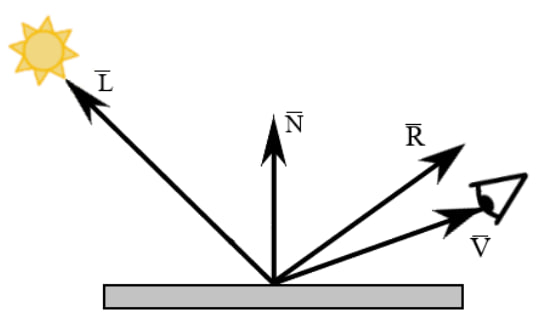
\includegraphics[width=.5\textwidth]{fong.jpg}
    \caption{Модель освещения Фонга}
    \label{fig:fong}
\end{figure}

На этом рисунке:
\begin{itemize}
    \item $\vec{L}$ --- вектор от точки на поверхности до источника света;
    \item $\vec{N}$ --- вектор нормали к поверхности в данной точке; 
    \item $\vec{R}$ --- вектор отражённого света;
    \item $\vec{V}$ --- вектор от точки на поверхности до наблюдателя (камеры);
\end{itemize}

Тогда интенсивность пикселя, отображающего данную точку на экране будет вычисляться согласно уравнению~\ref{eq:intens}.

\begin{equation}
    I = I_p \cdot K_a + I_0 \cdot K_b \cdot cos(\vec{L}, \vec{N}) + I_0 \cdot K_c \cdot cos^\alpha(\vec{R}, \vec{V})  
    \label{eq:intens}
\end{equation}

где $I$~---~итоговая интенсивность пикселя, отображающего данную точку на экране, $I_p$~---~интенсивность рассеянного света, $I_0$~---~интенсивность источника света, $K_a, K_b, K_c$~---~коэффициенты рассеянного, диффузного и зеркального освещения соответственно, $\alpha$~---~коэффициент блеска. 

$K_a, K_b, K_c, \alpha$ являются параметрами поверхности и, соответственно, константами. 

$I_p, K_a$ --- параметры модели освещения и тоже являются константами.

\subsection{Модель с картами освещения}

Модель с картами освещения --- это метод ускорить вычисления интенсивности освещения путём вычисления большинства параметров в момент построения сцены~\cite{LightMaps}. Такая модель может работать только в сценах, где положение объектов и источника(ов) освещения статичны. Сам метод сильно похож на метод теневых карт, однако вместо сохранения освещённости области изображения, будут сохранены значения векторов падающих на поверхность (и отражённых) лучей. 

Этот метод можно использовать вместе с моделью Фонга, чтобы значительно ускорить визуализацию очередного кадра.

Карту освещения, как и карту теней, придётся рассчитывать заново только если переместится источник света. В этот момент можно будет рассчитать все слагаемые из формулы~\ref{eq:intens} кроме последнего, а в последнем слагаемом останется рассчитать лишь косинус угла между векторами.

\subsection{Вывод}

В этой работе я буду использовать модель освещения Фонга с ускорением, использующим метод карт освещения. Поскольку построение реалистичного изображения не является целью работы, использовать более сложные (глобальные) модели освещения не нужно.

\clearpage

\def\bibname{\begin{center}\Large СПИСОК ИСПОЛЬЗОВАННЫХ ИСТОЧНИКОВ\end{center}}

\addcontentsline{toc}{chapter}{СПИСОК ИСПОЛЬЗОВАННЫХ ИСТОЧНИКОВ}
\begin{thebibliography}{}
  \bibitem{CGPaP} John F. Hugens. Computer Graphics Principles and Practice // 3-е издание // Бостон: Addison Wesley Professional // 1263 страницы

  \bibitem{QWFC} Heese, Raoul. Quantum Wave Function Collapse for Procedural Content Generation // статья // Institute of Electrical and Electronics Engineers (IEEE) // 13 страниц

  \bibitem{Rogers} Д. Роджерс Алгоритмические основы машинной графики // Перевод С.А. Вичес // Москва: Мир 1989г. // 512 страниц 

  \bibitem{Shadows} А.В. Мальцев Моделирование теней в 3D сценах с помощью каскадных теневых карт в режиме реального времени // статья // Журнал ИНФОРМАЦИОННЫЕ ТЕХНОЛОГИИ И ВЫЧИСЛИТЕЛЬНЫЕ СИСТЕМЫ // Москва: Российская Академия Наук 2014г. // 52 страницы

  \bibitem{LightMaps} Michael Abrash. Quake's lighting model: Surface caching. // Онлайн-ресурс: https://www.bluesnews.com/abrash/chap68.shtml // дата обращения: 03.11.2004

  % \bibitem{python3-matplotlib} Документация библиотеки Matplotlib: Visualization with Python /  [Электронный ресурс] // Matplotlib : [сайт]. — URL: https://matplotlib.org/ (дата обращения: 25.09.2024).

  % \bibitem{itmo-levenstein} Романовский И.В. Дискретный : Учебное пособие для студентов, специализирующихся по прикладной маткматике и информатике. // 4-е издание, исправленное и дополненное. // СПб.: Невский диалект; БХВ-Петербург, 2008. // 336 страниц

\end{thebibliography}

\end{document}